%kelompok 2 GIS (Ptolemy)
%Tiara Rizki Wulansari (1154026)
% Muhamad Rifan Zamaludin (1154088)
% Mohammad Agung Deomartha (1154032)
% M. Fajri Mualim (1154078)
% Faisal Syarifuddin

\section{Peta}
	peta adalah/merupakan penggambaran secara grafis atau bentuk skala (perbandingan) pada konsep mengenai bumi. dalam hal ini peta merupakan alat untuk menyampaikan atau menginformasikan mengenai ilmu kebumian. bagaimana peta dahulu ditemukan ? pengetahuan mengenai dasar pembentukan peta sama seperti filosofi, yang mana sering terdapat perbedaan.

\subsection{Peta Menurut Claudius Ptolemaeus Ptolemy}
	\begin{figure} [ht]
	\centerline{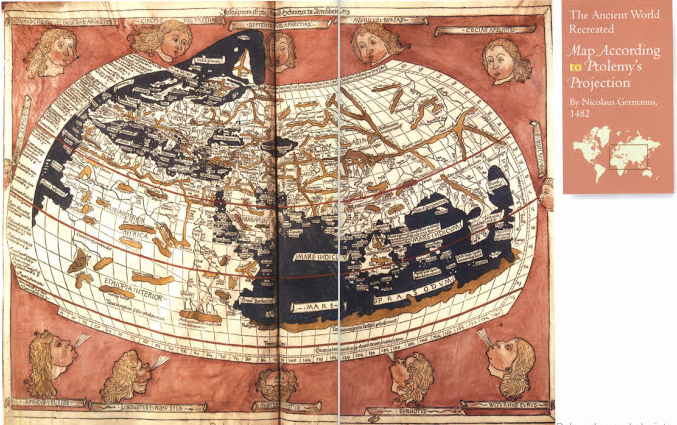
\includegraphics[width=.5\textwidth]{figures/PetaPtolemy}}
	\caption{Gambar Peta menurut Ptolemy}
	\label{PetaPtolemy}
	\end{figure}
	Gambar \ref {PetaPtolemy} Berikut adalah gambar dari Peta yang dibuat oleh Claudius Ptolemy.
	Claudius Ptolemaues yang dikenal dengan nama Ptolemy, hidup antara tahun 100 M dan 168 M, beliau merupakan salah satu sarjana sains pada masanya. Dia tinggal dan bekerja di Alexandria, kota Mesir yang merupakan pusat Intelektual dunia barat dengan perpustakaan paling luas yang pernah diciptakan. Ptolemy membawa semua pengetahuan dan keterampilan matematika dan astronomi dan menerapkannya pada pembuatan peta. Dia memiliki daya tarik matematikawan dengan presisi untuk menunjukkan hubungan satu tempat ke tenpat lain. Berdasarkan perhitungan lingkaran dunia 18.000 mil, ia juga mengembangkan sistem grid latude dan longtude yang dirancang oleh Marinus of Tire. sementara beberapa rincian peta mungkin sedikit aneh dengan garis lintang sejajar dengan garis khatulistiwa dengan garis bujur yang membentang ke utara-selatan dengan busur anggun, sudah tidak asing lagi bagi siapa saja yang pernah memiliki atlas. dalam kerangka ini, ptolemy mampu membangun koordinat dan mendaftarkan lebih dari 8000 tempat dengan koordinat masing-masing. Bagi ptolemy, ini adalah latihan matematik dan kita tidak akan pernah tahu apakah dia benar-benar menggambar peta dari sini.
	Data-data tentang Pembuatan peta sempat hilang ketika perpustakaan Alexandria yang terkenal dibakar oleh orang-orang kristen fanatik pada tahun 390 Masehi - sebuah contoh awal konflik antara iman dan sains. Tapi setidaknya satu salinan yang telah dibuat dari karya Ptolemy terselamatkan dan ini bertahan di Byzantium. 1000 tahun berlalu dan kemudian tulisannya digunakan untuk dikembangkan oleh ilmuwan Arab, sementara di bagian eropa tetap dalam ketidaktahuan akan warisannya. Baru pada saat renaisans muncul di italia dan daya tarik di dunia, Geografi Ptolemy diterjemahkan dalam bahasa Latin dan gagasannya terhadap PETA Duniadapat diakses oleh para ilmuwan.
	Namun tidak ada peta dalam keadaan masih utuh, hanya petunjuk dan saran untuk pembuatan map dan daftar koordinat \cite{smart2005maps}.
	\begin{figure} [ht]
	\centerline{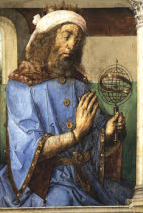
\includegraphics[width=.5\textwidth]{figures/ptolemy}}
	\caption{Foto Ptolemy}
	\label{ptolemy}
	\end{figure}
	gambar \ref{ptolemy} Foto Ptolemy seorang ahli astronomi, geografi, matematikawan.

\subsection{Peta Dunia Ptolemy}
		Peta dunia Ptolemy adalah peta gambaran dunia yang diketahui masyarakat barat pada kurun kedua masihi.Peta tersebut berdasarkan penerangan yang terkandung di dalam buku Geographia, ditulis kira-kira pada 150 masehi. walaupun peta autentik tidak dijumpai, buku Geographia yng mengandungi beribu-ribu rujukan pelbagai tempat di dunia lama, berserta kordinat, yang membolehkan para pelukis peta menyusun semula peta dunia Ptolemy apabila manuskriptnya telah ditemui sekitar 1300 masihi.
	\begin{figure} [ht]
	\centerline{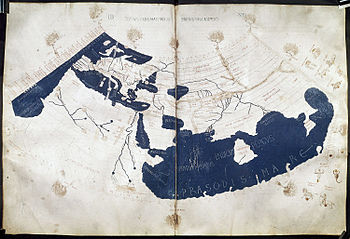
\includegraphics[width=.5\textwidth]{figures/PtolemyWorldMap}}
	\caption{Gambar Ptolemy}	
	\label{PtolemyWorldMap}
	\end{figure}
	gambar \ref {PtolemyWorldMap} Peta Dunia Ptolemy, disusun semula dari Geographia Ptolemy (kira-kira 150) pada kurun ke 15, menunjukan Sinae (China) di sebelah kanan, di bawah pulau Taprobane (Sri Lanka, diperbesarkan) dan Aurea Chersonesus (Semenanjung Asia Tenggara).

	\begin{figure} [ht]
	\centerline{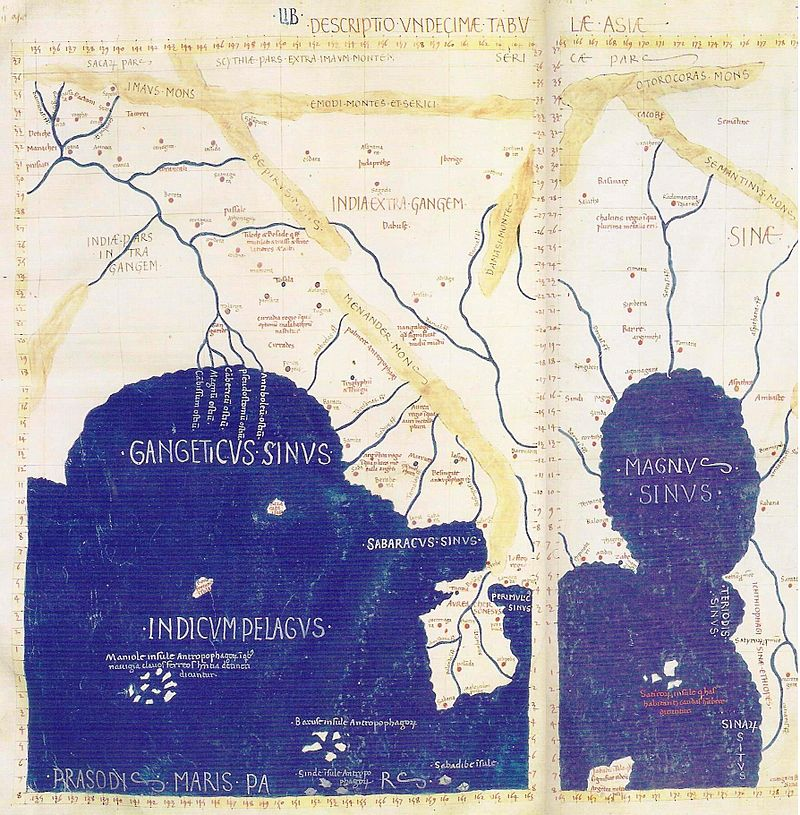
\includegraphics[width=.5\textwidth]{figures/PtolemyAsiadetail}}	
	\caption{Gambar Perincian Timur dan Asia}
	\label{PtolemyAsiadetail}		
	\end{figure}
	Gambar \ref{PtolemyAsiadetail} adalah perinician Timur dan Asia Tenggara dalam peta dunia Ptolemy.Teluk Ganges (Teluk Bengali) kiri, Semenanjung Asia Tenggara di tengah, Laut China selatan kanan, bersama Sinae (China).
	
\subsection{Sejarah Ptolemy}
	\begin{figure} [ht]
	\centerline{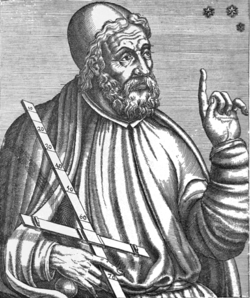
\includegraphics[width=.5\textwidth]{figures/Ptolemyporg}}
	\caption{Konsep artis zaman pertengahan dari Claudius Ptolemaeus.}
	\label{Ptolemyporg}
	\end{figure}
    Gambar \ref{Ptolemyporg} adalah Claudius Ptolemaeus (90 – 168), adalah seorang ahli geografi, astronom, dan astrolog yang hidup pada zaman Helenistik di provinsi Romawi, Aegyptus.
    Ptolemaeus adalah pengarang beberapa risalah ilmiah, tiga di antaranya kemudian memainkan peranan penting dalam keilmuwan Islam dan Eropa. Yang pertama adalah risalah astronomi yang dikenal sebagai Almagest (dalam bahasa Yunani Η μεγάλη Σύνταξις , Risalah Besar). Yang kedua adalah Geographia, yang merupakan diskusi teliti mengenai pengetahuan geografi Helenistik. Yang ketiga adalah risalah astrologi dikenal sebagai Tetrabiblos (Empat buku) di mana dia berusaha mengadaptasi astrologi horoskop ke filosofi alam Aristotelian. Ia juga melestarikan daftar raja-raja kuno, disebut Kanon Ptolemaeus, yang penting bagi penelitian sejarah Timur Tengah.
    Claudius adalah nomen (nama keluarga) seorang Roma; Ptolemaeus menyandang nama itu, sehingga menjadi bukti bahwa dia adalah seorang warganegara Roma. Sesuai kebiasaan, Keluarga Ptolemy pertama yang menjadi warganegara (entah itu dia atau nenek moyangnya) mengambil nama itu dari seorang Roma yang bernama Claudius, sehingga membuatnya diberi status kewarganegaraan. Jika orang Roma ini adalah kaisar, kewarganegaraan sudah akan diberi di antara tahun 41 dan 68 M. (waktu Claudius, lalu Nero, menjabat kaisar). Astronom itu juga mempunyai praenomen (nama pertama), yang tetap tak diketahui. Tetapi, kemungkinan Tiberius, karena praenomen itu sangat umum di antara yang keluarga-keluarga yang diberi kewarganegaraan oleh kaisar ini.
    Ptolemaeus (Ptolemy) adalah sebuah nama Yunani. Muncul satu kali di mitologi Yunani, dalam bentuk Homeric. Cukup biasa di antara golongan sol bagian atas Makedonia pada saat Alexander Agung, dan ada beberapa di antara tentara Alexander, satu di antaranya pada tahun 323 S.M. menjadikan dirinya sendiri Raja Mesir: Ptolemy I Soter; semua raja setelah dia, sampai Mesir menjadi provinsi Roma pada tahun 30 S.M., adalah juga dari dinasti Ptolemaic. Hanya ada sedikit bukti tentang subyek asal usul Ptolemy (meskipun melihat di atas kewarganegaraan Roma keluarganya), tetapi kebanyakan sarjana dan sejarawan mempertimbangkannya tak mungkin bahwa Ptolemeus berhubungan dengan dinasti kerajaan Ptolemies.
    Selain dianggap sebagai seorang anggota masyarakat Yunani Alexandria, hanya sedikit rincian hidup Ptolemaeus yang diketahui. Dia menulis dalam bahasa Yunani Kuno dan diketahui sudah menggunakan data astronomis Babilonia.Seorang warganegara Roma, beberapa sarjana menyimpulkan bahwa secara etnik, Ptolemeus adalah orang Yunani, dan sarjana lainnya berpendapat bahwa dia secara etnik orang Mesir, meskipun Hellenize. Dia banyak dikenal dalam sumber bahasa Arab yang muncul kemudian sebagai Upper Egyptian, diperkirakan dia mungkin berasal dari Mesir selatan. Astronom, ahli ilmu bumi, dan pakar fisika Arab selanjutnya merujuk padanya menggunakan nama Arabnya Batlamyus.
    Karya utama Ptolemy lainnya adalah Geografinya (juga disebut Geographia), kompilasi koordinat geografis dari bagian dunia yang dikenal oleh Kekaisaran Romawi pada masanya. Dia agak bergantung pada karya seorang ahli geografi sebelumnya, Marinos of Tire, dan pada kano Romawi dan Kekaisaran Persia kuno. [Rujukan] Dia juga mengakui astronom Hipparchus kuno karena telah menyediakan ketinggian kutub utara untuk beberapa kota.[19]
  
  \subsection{The Geography}	
   \begin{figure} [ht]
	\centerline{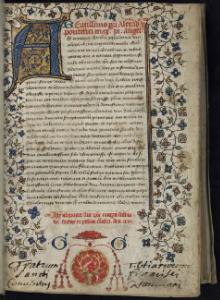
\includegraphics[width=.5\textwidth]{figures/geography}}
	\caption{Geography by Ptolemy}
	\label{geography}
		\end{figure}
    gambar \ref {geography} Bagian pertama dari Geografi adalah diskusi tentang data dan metode yang dia gunakan. Seperti model tata surya di Almagest, Ptolemy memasukkan semua informasi ini ke dalam skema besar. Setelah Marinos, dia memberikan koordinat ke semua tempat dan fitur geografis yang dia ketahui, dalam kotak yang membentang di seluruh dunia. Lintang diukur dari khatulistiwa, seperti sekarang, tapi Ptolemy lebih suka [20] untuk mengekspresikannya sebagai climata, panjang hari terpanjang daripada deretan busur: panjang hari senin mulai meningkat dari 12h menjadi 24 jam saat seseorang pergi. dari khatulistiwa ke lingkaran kutub. Dalam buku 2 sampai 7, dia menggunakan gelar dan meletakkan garis meridian 0 bujur di tanah paling barat yang dia kenal, Kepulauan Terberkati, yang sering diidentifikasi sebagai Kepulauan Canary, seperti yang disarankan oleh lokasi dari enam titik yang diberi label FORTUNATA pulau-pulau di dekat ekstrem kiri laut biru peta Ptolemeus di sini direproduksi.
	Ptolemeus juga merancang dan memberikan petunjuk bagaimana membuat peta di seluruh dunia yang berpenghuni (oikoumenè) dan provinsi Romawi. Di bagian kedua Geografi, dia memberikan daftar topografi yang diperlukan, dan teks untuk peta. Oikoumenènya membentang 180 derajat bujur dari Kepulauan Terberkati di Samudra Atlantik sampai ke Cina tengah, dan sekitar 80 derajat garis lintang dari Shetland menjadi anti-Meroe (pantai timur Afrika); Ptolemy sangat sadar bahwa dia tahu tentang hanya seperempat dunia, dan perpanjangan yang salah dari Cina ke selatan menunjukkan sumbernya tidak sampai ke Samudra Pasifik.
	Peta di manuskrip yang masih ada di Ptolemy's Geography, bagaimanapun, hanya berasal dari sekitar tahun 1300, setelah teks tersebut ditemukan kembali oleh Maximus Planudes. Tampaknya tabel topografi dalam buku 2-7 adalah teks kumulatif - teks yang diubah dan ditambahkan sebagai pengetahuan baru yang tersedia di abad setelah Ptolemy. [21] Ini berarti bahwa informasi yang terdapat di berbagai bagian Geografi kemungkinan berasal dari tanggal yang berbeda. 
	Peta berdasarkan prinsip ilmiah telah dibuat sejak zaman Eratosthenes, pada abad ke-3 SM, namun Ptolemy memperbaiki proyeksi peta. Diketahui dari sebuah pidato oleh Eumenius bahwa peta dunia, sebuah orbis pictus, yang tidak diragukan lagi berdasarkan Geografi, dipajang di sebuah sekolah di Augustodunum, Gaul pada abad ketiga. [22] Pada abad ke-15, Geografi Ptolemy mulai dicetak dengan peta terukir; edisi cetak paling awal dengan peta terukir diproduksi di Bologna pada 1477, diikuti dengan cepat oleh edisi Romawi tahun 1478 (Campbell, 1987). Sebuah edisi yang dicetak di Ulm pada tahun 1482, termasuk peta tebing kayu, adalah yang pertama dicetak di utara Pegunungan Alpen. Peta terlihat terdistorsi bila dibandingkan dengan peta modern, karena data Ptolemy tidak akurat. Salah satu alasannya adalah Ptolemy memperkirakan ukuran Bumi terlalu kecil: sementara Eratosthenes menemukan 700 stadion untuk sebuah lingkaran besar di dunia, Ptolemy menggunakan 500 stadion di Geografi. Sangat mungkin bahwa ini adalah stadion yang sama, karena Ptolemy beralih dari skala sebelumnya ke yang terakhir antara Syntaxis dan Geography, dan menyesuaikan derajat bujur yang sesuai. Lihat juga unit pengukuran dan Sejarah Yunani Kuno geodesi.
	Karena Ptolemy berasal dari garis lintang utamanya dari nilai terpanjang minyak mentah, garis lintangnya rata-rata keliru kira-kira satu derajat (2 derajat untuk Bizantium, 4 derajat untuk Kartago), meskipun para astronom kuno mampu mengetahui garis lintang mereka lebih lama. (Lambang Ptolemeus sendiri salah oleh 14.) Dia setuju (Geografi 1.4) bahwa bujur paling baik ditentukan oleh observasi simultan gerhana bulan, namun dia sangat tidak berhubungan dengan ilmuwan pada masanya bahwa dia tidak mengetahui data semacam itu. lebih baru dari 500 tahun sebelumnya (Arbela gerhana). Ketika beralih dari 700 stadia per derajat ke 500, dia (atau Marinos) memperluas perbedaan bujur antara kota-kota yang sesuai (sebuah titik yang pertama kali direalisasikan oleh P.Gosselin pada tahun 1790), yang mengakibatkan peregangan skala bumi timur-barat yang serius dalam derajat, meski tidak jauh. Mencapai garis bujur yang sangat tepat tetap menjadi masalah dalam geografi sampai penerapan metode bulan Jovian Galileo di abad ke-18. Harus ditambahkan bahwa daftar topografinya yang asli tidak dapat direkonstruksi: tabel panjang dengan angka dikirim ke anak cucu melalui salinan yang mengandung banyak kesalahan juru tulis, dan orang selalu menambahkan atau memperbaiki data topografi: ini adalah kesaksian akan popularitas yang terus-menerus dari Karya ini berpengaruh dalam sejarah kartografi.

